% !TeX root = main.tex
\chapter{Functional Analysis and System Architecture}

\section*{Introduction}
\addcontentsline{toc}{section}{Introduction}

This chapter presents the architectural analysis of Football OS and relates the
functional constraints to service decomposition, inter-module communication,
and the security strategy.

\section{Functional Analysis Synthesis}
The business needs and use cases detailed in Chapter~1 are translated here
into architectural decisions: centralized access through the Gateway,
separation between Governance and Workspace responsibilities, and controlled
externalization of authorization policies.

\section{Global System Architecture}

\subsection{Architectural Style and Decision Analysis}

Football OS adopts a microservices-oriented architecture organized inside a
monorepo. The system is not implemented as a single monolithic backend: the
API Gateway, Governance Service, and Workspace Service are separated as
distinct backend applications with their own responsibilities, runtime
configuration, and persistence concerns. The monorepo structure was kept to
simplify development, dependency management, and Shared SDK evolution during
the internship.

This choice provides a compromise between a simple monolith and a fully
distributed multi-repository microservices ecosystem. A monolith would have
reduced deployment complexity but would have mixed governance, workspace
operations, authorization, and document workflows inside one application. A
fully independent multi-repository microservices organization would have
increased operational overhead, CI/CD complexity, and version-management cost.
The selected architecture keeps clear service boundaries while remaining
manageable for a small-team academic project.

Classic SOA is retained in this report only as a comparison baseline, while the
implemented backend aligns with a microservices-oriented monorepo model
\cite{soa-erl,microservices-newman}. Backend service internals still follow
Onion/Clean Architecture layering to keep domain logic isolated from technical
adapters \cite{clean-arch}.

\begin{table}[ht]
\centering
\caption{Architecture decision matrix}
\label{tab:architecture-decision-matrix}
\small
\setlength{\tabcolsep}{3pt}
\renewcommand{\arraystretch}{1.08}
\begin{tabularx}{\textwidth}{|L{3.0cm}|C{1.8cm}|C{1.8cm}|C{2.5cm}|Y|}
\hline
\textbf{Criterion} & \textbf{Monolith} & \textbf{Classic SOA} & \makecell[c]{\textbf{Multi-repository}\\\textbf{Microservices}} & \makecell[c]{\textbf{Selected}\\\textbf{Microservices Monorepo}} \\
\hline
Maintainability & Medium & Medium & High & High \\
\hline
\makecell[l]{Deployment\\complexity} & Low & Medium & High & Medium \\
\hline
Domain ownership & Low & Medium & High & High \\
\hline
Security isolation & Medium & Medium & High & High \\
\hline
\makecell[l]{Team-size\\suitability} & High (small team) & Medium & Low (small team) & High (small team) \\
\hline
Latency overhead & Low & Medium & High & Medium \\
\hline
\makecell[l]{Shared code\\management} & \makecell[c]{Simple but\\coupled} & Moderate & \makecell[c]{Difficult\\across repos} & \makecell[c]{Centralized\\and controlled} \\
\hline
\end{tabularx}
\normalsize
\end{table}

The selected option is therefore not a classic centralized SOA model, but a
microservices-oriented monorepo. Gateway owns edge enforcement, Governance owns
identity/canonical/policy/audit concerns, Workspace owns operational document,
event, profile, and notification workflows, and the Shared SDK reduces
duplicated integration code while preserving service-level separation.

\subsection{Architecture Overview}

The architecture diagram below situates how frontend requests are funneled
through the Gateway and then distributed across governance and workspace
responsibilities, while shared SDK modules and infrastructure services provide
cross-cutting technical support.

\begin{figure}[ht]
    \centering
    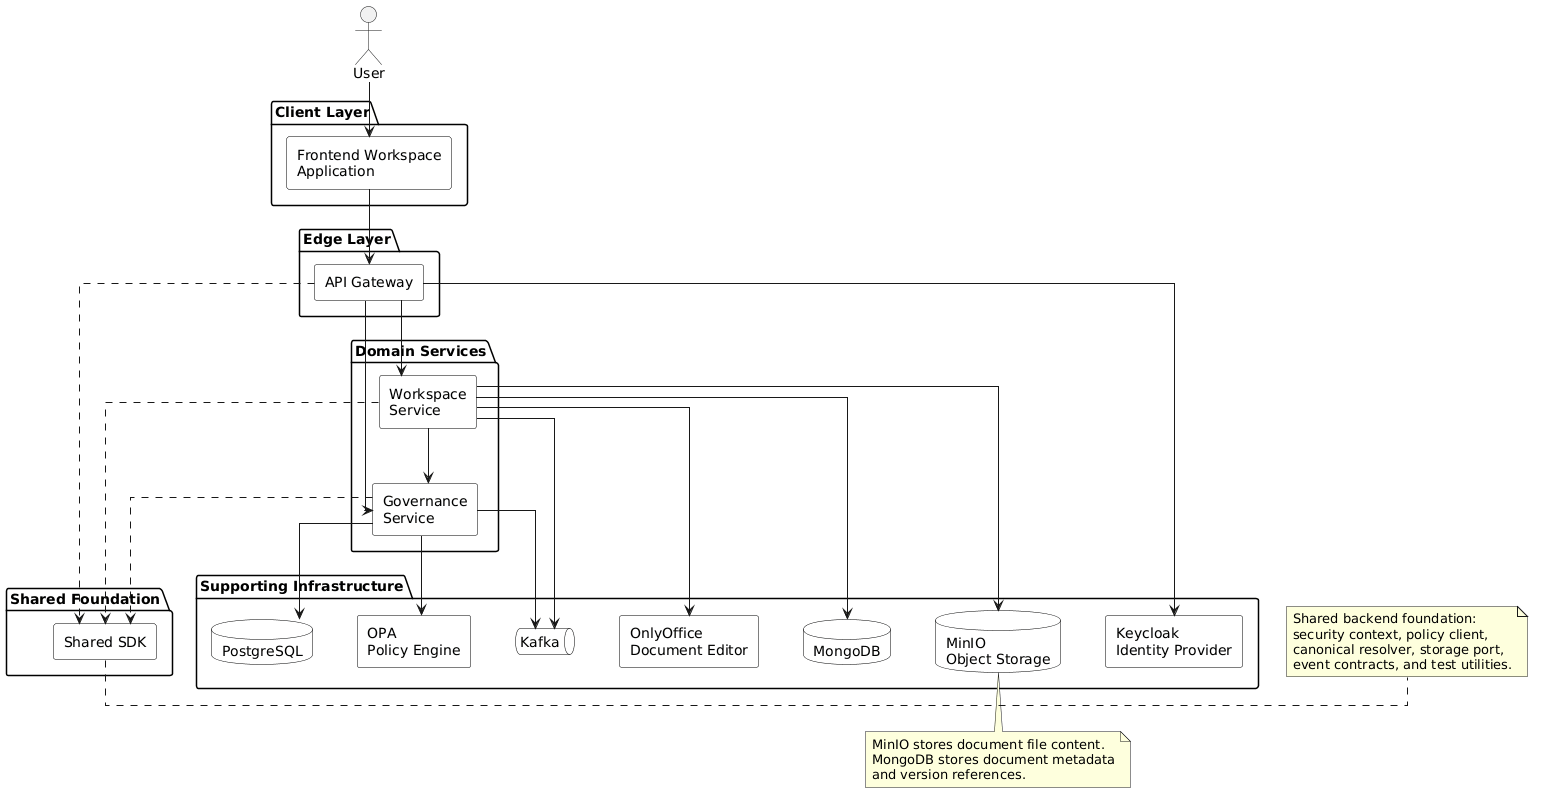
\includegraphics[width=0.95\textwidth]{images/architecture-logique.png}
    \caption{Global architecture of the Football OS platform}
    \label{fig:global-architecture}
\end{figure}

Figure~\ref{fig:global-architecture} highlights a deliberate boundary: client
applications are decoupled from internal service topology. Routing and edge
controls are centralized at the Gateway, while Governance and Workspace evolve
behind stable API contracts. This decision reduced frontend-backend coupling at
the price of adding an intermediate network hop and stronger dependency on
Gateway availability.

The infrastructure layer supports persistence, messaging, policy evaluation,
storage, and document editing. Asynchronous exchanges were introduced where
traceability and propagation mattered more than immediate synchronous response
time, in line with event-driven integration principles \cite{eda-fowler}.

\begin{table}[ht]
\centering
\caption{Default local entry points used during development}
\label{tab:local-entry-points}
\begin{tabular}{|p{4.5cm}|p{3cm}|p{6.5cm}|}
\hline
\textbf{Component} & \textbf{Port} & \textbf{Access role} \\
\hline
Workspace Frontend & 4200 & User web interface. \\
\hline
API Gateway & 8080 & Public backend entry point for frontend API calls. \\
\hline
Governance Service & 8081 & Internal/backend endpoint behind Gateway routing. \\
\hline
Workspace Service & 8082 & Internal/backend endpoint behind Gateway routing. \\
\hline
\end{tabular}
\end{table}

Table~\ref{tab:local-entry-points} clarifies that frontend API traffic goes
through the Gateway rather than directly to internal services.

\subsection{Main Components}

\begin{table}[ht]
\centering
\caption{Main components of the Football OS architecture}
\label{tab:main-components}
\small
\setlength{\tabcolsep}{4pt}
\renewcommand{\arraystretch}{1.10}
\begin{tabularx}{\textwidth}{|L{3.7cm}|Y|L{3.3cm}|}
\hline
\textbf{Component} & \textbf{Responsibility} & \textbf{Main Technology} \\
\hline
Frontend Workspace Application & User interface for workspace operations and platform access. & Angular + Tailwind CSS \\
\hline
API Gateway & Entry point of backend APIs; routes requests and enforces secure access flow. & Spring Boot (Gateway layer) \\
\hline
Governance Service & Manages users, roles, permissions, canonical players/teams, policy decisions, and audit tracking. & Spring Boot + PostgreSQL + OPA \\
\hline
Workspace Service & Manages documents, calendar/events, notifications, search, and player profile aggregation. & Spring Boot + MongoDB + MinIO \\
\hline
Shared SDK & Shared foundation/library used by backend services; provides reusable abstractions and common integration mechanisms. & Java multi-module SDK \\
\hline
Keycloak / Identity Provider & Authenticates users and provides identity context. & Keycloak (OIDC/JWKS) \\
\hline
OPA Policy Engine & Evaluates authorization rules for protected actions and resources. & Open Policy Agent \\
\hline
Kafka & Supports asynchronous event messaging and notification propagation. & Apache Kafka \\
\hline
PostgreSQL & Stores governance structured data such as actors, roles, players, teams, and audit logs. & PostgreSQL \\
\hline
MongoDB & Stores workspace aggregates and document metadata/version references, including documents, events, and notifications. & MongoDB \\
\hline
MinIO & Stores the actual document file content and file versions. & MinIO Object Storage \\
\hline
Redis & Supports Gateway-level rate limiting and request throttling. & Redis \\
\hline
OnlyOffice & Enables online document viewing and editing workflows. & OnlyOffice Docs \\
\hline
\end{tabularx}
\normalsize
\end{table}

The component matrix makes explicit that each subsystem is mapped to a dominant
responsibility domain, which improves maintainability and ownership clarity.
The same decomposition also introduces integration overhead, especially where
authorization, identity context, and cross-store references intersect.

\section{Backend Module Design}

\subsection{API Gateway}

The API Gateway is the backend entry point. It validates token context, applies
edge controls, and routes requests to Governance and Workspace without exposing
internal service addresses.

Compared with direct client-to-service exposure, this Gateway-mediated model
improves policy consistency and request normalization. The trade-off is that
the Gateway becomes a critical dependency that must be monitored and configured
carefully to avoid becoming a bottleneck.

\subsection{Governance Service}

The Governance Service owns actor/role management, canonical players/teams,
policy decision support through OPA, and audit traceability data.

This separation was chosen to keep authorization and identity logic outside
feature modules. It simplifies compliance reasoning and avoids scattered access
rules, but it also increases inter-service calls whenever Workspace operations
require policy checks or canonical references.

\subsection{Workspace Service}

The Workspace Service owns operational modules (documents, events,
notifications, search, and profile aggregation), persists workspace aggregates
in MongoDB, and integrates with Governance, MinIO, Kafka, and OnlyOffice.

The module boundary favors business-flow cohesion: operational features evolve
in one service while governance remains externalized. The main limitation is
coordination complexity for workflows that span metadata, policy, storage, and
messaging components.

\subsection{Shared SDK}

The Shared SDK is not a user-facing module. It is reused by backend services to
avoid duplicated technical plumbing. It provides shared security context,
policy client, canonical resolver, storage port abstraction, event contracts,
audit hooks, and test utilities.

In implementation terms, the SDK is structured as real backend submodules
rather than a generic helper package. Table~\ref{tab:sdk-submodules} outlines
the modules used by Governance and Workspace services.

\begin{table}[H]
\centering
\caption{Shared SDK submodules and engineering roles}
\label{tab:sdk-submodules}
\small
\setlength{\tabcolsep}{4pt}
\renewcommand{\arraystretch}{1.10}
\begin{tabularx}{\textwidth}{|L{2.7cm}|Y|}
\hline
\textbf{Submodule} & \textbf{Role in the platform} \\
\hline
\texttt{sdk-core} & Shared primitives, base entities/documents, lifecycle states, and common response models. \\
\hline
\texttt{sdk-events} & Signal envelope, Kafka topics, producer/consumer patterns, and correlation context contracts. \\
\hline
\texttt{sdk-security} & Authenticated actor context, role extraction, JWT-related helpers, and audit hooks. \\
\hline
\texttt{sdk-storage} & Storage abstraction layer that decouples services from MinIO-specific details and supports future provider evolution. \\
\hline
\texttt{sdk-canonical} & Canonical player/team references and resolver/client mechanisms used by workspace workflows. \\
\hline
\texttt{sdk-policy} & Policy request/result contracts, policy client integration, and method-level guard support. \\
\hline
\texttt{sdk-test} & Reusable integration-test utilities and shared test support components. \\
\hline
\end{tabularx}
\normalsize
\end{table}

Using a shared SDK reduced repeated integration code and aligned conventions
across services. The associated risk is version coupling: service teams must
coordinate SDK evolution to avoid incompatible upgrades.

\subsection{Service Responsibility Summary}

\begin{table}[ht]
\centering
\caption{Service boundary summary}
\label{tab:module-responsibility}
\small
\setlength{\tabcolsep}{4pt}
\renewcommand{\arraystretch}{1.10}
\begin{tabularx}{\textwidth}{|L{2.8cm}|Y|L{2.2cm}|Y|}
\hline
\textbf{Service / Module} & \textbf{Ownership} & \textbf{Persistence} & \textbf{Main integrations} \\
\hline
API Gateway & Edge security, request enrichment, rate limiting, and routing to backend services. & No business DB & Keycloak JWKS, Redis, Governance Service, Workspace Service \\
\hline
Governance Service & Actors, roles, canonical players/teams, policy evaluation flow, and audit ownership. & PostgreSQL & OPA, Kafka, Keycloak, Shared SDK \\
\hline
Workspace Service & Documents, events, profiles, notifications, search, and OnlyOffice-related workflows. & MongoDB + MinIO & Governance policy/canonical APIs, Kafka, OnlyOffice \\
\hline
Shared SDK & Shared contracts and reusable adapters for security, policy, canonical, storage, events, and tests. & No business DB & Security, policy, canonical, storage, events, tests \\
\hline
\end{tabularx}
\normalsize
\end{table}
Table~\ref{tab:module-responsibility} consolidates the separation of
responsibilities across backend modules.

\subsection{API Summary}

Table~\ref{tab:api-summary} provides a compact overview of representative
endpoint families used by the platform.

\begin{table}[H]
\centering
\caption{API endpoint family summary}
\label{tab:api-summary}
\small
\renewcommand{\arraystretch}{1.10}
\setlength{\tabcolsep}{4pt}
\begin{tabularx}{\textwidth}{|L{2.4cm}|L{3.8cm}|Y|}
\hline
\textbf{Module} & \textbf{Endpoint family} & \textbf{Purpose} \\
\hline
Workspace & \makecell[l]{\texttt{/api/v1/}\\\texttt{documents}} & Document upload, consultation, categorization, and lifecycle operations. \\
\hline
Workspace & \makecell[l]{\texttt{/api/v1/}\\\texttt{events}} & Event creation, consultation, update, and archive workflows. \\
\hline
Workspace & \makecell[l]{\texttt{/api/v1/}\\\texttt{profiles}} & Role-filtered player profile consultation and aggregation. \\
\hline
Workspace & \makecell[l]{\texttt{/api/v1/}\\\texttt{notifications}} & Notification generation, retrieval, and state updates. \\
\hline
Workspace & \makecell[l]{\texttt{/api/v1/}\\\texttt{search}} & Search across workspace resources with access filtering. \\
\hline
Workspace & \makecell[l]{\texttt{/api/v1/}\\\texttt{onlyoffice}} & Online document editor integration and callback-related actions. \\
\hline
Governance & \makecell[l]{\texttt{/api/v1/}\\\texttt{actors}} & Actor management and actor-role relationship management. \\
\hline
Governance & \makecell[l]{\texttt{/api/v1/}\\\texttt{players}} & Canonical player data operations and references. \\
\hline
Governance & \makecell[l]{\texttt{/api/v1/}\\\texttt{teams}} & Canonical team data operations and references. \\
\hline
Governance & \makecell[l]{\texttt{/api/v1/}\\\texttt{policy}} & Authorization decision endpoints for protected actions. \\
\hline
\end{tabularx}
\normalsize
\setlength{\tabcolsep}{6pt}
\end{table}

Rather than exposing database structures, these interfaces are organized around
business actions (document lifecycle, event coordination, profile consultation,
policy evaluation). This orientation improves API stability and limits
frontend dependence on persistence internals.

\subsection{Critical Review of Service Decomposition}

The decomposition solved a practical project constraint: maintaining clear
ownership while delivering heterogeneous workflows in a limited internship
timeline. Compared with a monolith, this approach improved modularity and
change isolation. Compared with fully independent repositories, it reduced
coordination overhead through a shared codebase and SDK.

The remaining constraint is operational complexity. Service boundaries are
useful only if integration contracts, failure handling, and deployment
discipline remain explicit; these points represent the principal engineering
workload for future iterations.



\section{Security and Authorization Architecture}

Football OS combines identity-provider authentication, Gateway-level token
validation, policy-based authorization, and backend-side access checks. The
security model is designed so that the frontend improves usability but does not
become the final enforcement point for protected resources
\cite{keycloak-doc,oauth2-rfc6749,oidc-core,rbac-sandhu,opa-doc}.

\subsection{Security Implementation Details}

\begin{table}[!htbp]
\centering
\caption{Security implementation choices}
\label{tab:security-implementation-choices}
\footnotesize
\setlength{\tabcolsep}{4pt}
\renewcommand{\arraystretch}{1.14}
\begin{tabularx}{\textwidth}{|L{3.2cm}|Y|}
\hline
\textbf{Security concern} & \textbf{Implementation choice} \\
\hline
Authentication & Keycloak with OIDC and JWT-based access tokens. \\
\hline
Token validation & API Gateway validates access tokens using Keycloak JWKS through the resource-server security configuration. \\
\hline
Session model & Backend services remain stateless and rely on token-based authentication context. \\
\hline
Token propagation & The frontend sends a bearer token to the Gateway; the Gateway enriches/forwards actor context to downstream services. \\
\hline
Authorization & Workspace calls the Governance policy endpoint, which relies on OPA-backed decisions. \\
\hline
Rate limiting & Gateway-level Redis-backed rate limiting protects backend entry points from excessive requests. \\
\hline
File access & Document metadata and category are checked by policy before storage or editor access is generated. \\
\hline
Upload protection & Upload actions are constrained by authorization rules, document category, and role-based visibility. \\
\hline
CSRF exposure & Exposure is reduced because API calls use bearer-token authorization rather than cookie-based backend sessions. \\
\hline
CORS policy & In deployment, allowed origins should be restricted to the configured frontend origin. \\
\hline
\end{tabularx}
\normalsize
\end{table}

This design keeps security enforcement on the server side. Hidden buttons and
role-based interface states improve the user experience, but protected actions
are still checked by backend services before data, storage URLs, or editor
configurations are returned.

The choice of externalized policy evaluation through OPA was preferred over
hardcoded authorization checks scattered across services. This improves policy
traceability and change control, but introduces dependency on policy
availability and policy-model synchronization between governance and consuming
services.

\begin{table}[ht]
\centering
\caption{Access-control matrix for core platform actions}
\label{tab:access-control-matrix}
\footnotesize
\setlength{\tabcolsep}{4pt}
\renewcommand{\arraystretch}{1.14}
\begin{tabularx}{\textwidth}{|Y|C{2.1cm}|C{2.1cm}|C{2.1cm}|C{2.1cm}|}
\hline
\textbf{Resource / Action} & \textbf{Club Administrator} & \textbf{Head Coach} & \textbf{Coaching Staff} & \textbf{Medical Staff} \\
\hline
Manage users and roles & Allowed & Denied & Denied & Denied \\
\hline
Manage canonical players/teams & Allowed & Policy & Denied & Denied \\
\hline
Create/update/archive events & Denied & Allowed & Policy & Denied \\
\hline
Consult events & Allowed & Allowed & Allowed & Policy \\
\hline
Upload normal documents & Allowed & Allowed & Policy & Policy \\
\hline
Consult normal documents & Allowed & Allowed & Policy & Policy \\
\hline
Access medical documents & Restricted & Denied & Denied & Allowed \\
\hline
Access admin/contract documents & Allowed & Denied & Denied & Denied \\
\hline
Consult player profiles & Allowed & Allowed & Policy & Restricted \\
\hline
Receive notifications & Allowed & Allowed & Allowed & Allowed \\
\hline
\end{tabularx}
\normalsize
\end{table}

The access-control matrix captures the nominal role posture used as a policy
baseline. In operational execution, final authorization remains policy-based on
the backend.

Overall, the security design addresses the main project constraint of
centralized, auditable authorization across heterogeneous workflows. Its
principal limitation is operational: policy and Gateway layers require robust
observability and fallback handling to remain reliable under failure conditions.



\section*{Conclusion}
\addcontentsline{toc}{section}{Conclusion}

This architecture ensures a clear separation of responsibilities and preserves
security and governance coherence across the platform workflows.
